\documentclass[12pt]{article}
\usepackage[margin=1in]{geometry}  % set the margins to 1in on all sides
\usepackage{graphicx}              % to include figures
\usepackage{amsmath}               % great math stuff
\usepackage{amsfonts}              % for blackboard bold, etc
\usepackage{amsthm}                % better theorem environments
\usepackage{amsthm,amssymb}
\usepackage[hidelinks]{hyperref}
\usepackage{xcolor,cancel}
\newcommand\hcancel[2][black]{\setbox0=\hbox{$#2$}%
\rlap{\raisebox{.45\ht0}{\textcolor{#1}{\rule{\wd0}{1pt}}}}#2}

\newtheorem{thm}{Theorem}[section]
\newtheorem{lem}[thm]{Lemma}
\newtheorem{prop}[thm]{Proposition}
\newtheorem{cor}[thm]{Corollary}
\newtheorem{conj}[thm]{Conjecture}

\theoremstyle{definition}
\newtheorem{defn}[thm]{Definition}
\newtheorem{defns}[thm]{Definitions}
\newtheorem{con}[thm]{Construction}
\newtheorem{exmp}[thm]{Example}
\newtheorem{exmps}[thm]{Examples}
\newtheorem{notn}[thm]{Notation}
\newtheorem{notns}[thm]{Notations}
\newtheorem{addm}[thm]{Addendum}
\newtheorem{exer}[thm]{Exercise}

\DeclareMathOperator{\id}{id}

\newcommand{\bd}[1]{\mathbf{#1}}  % for bolding symbols
\newcommand{\RR}{\mathbb{R}}      % for Real numbers
\newcommand{\ZZ}{\mathbb{Z}}      % for Integers
\newcommand{\col}[1]{\left[\begin{matrix} #1 \end{matrix} \right]}
\newcommand{\comb}[2]{\binom{#1^2 + #2^2}{#1+#2}}
\usepackage{cleveref}	
\begin{document}


\nocite{}

\title{Applications of matrices}

\author{Miliyon T.}
\date{October 7, 2013}
\maketitle


\section{Area using matrices}
\begin{thm}
Given a triangle with vertices $(x_1,y_1),\ (x_2,y_2)$ and $(x_3,y_3)$, then the area of the given triangle is given by
\[ \frac{1}{2}\left|
    \begin{matrix}
      x_1 & y_1 & 1\\
      x_2 & y_2 & 1\\
      x_3 & y_3 & 1
    \end{matrix}
    \right|\]
\end{thm}
\begin{proof}
Consider the following figure
\begin{figure}[hbt!]
\centering
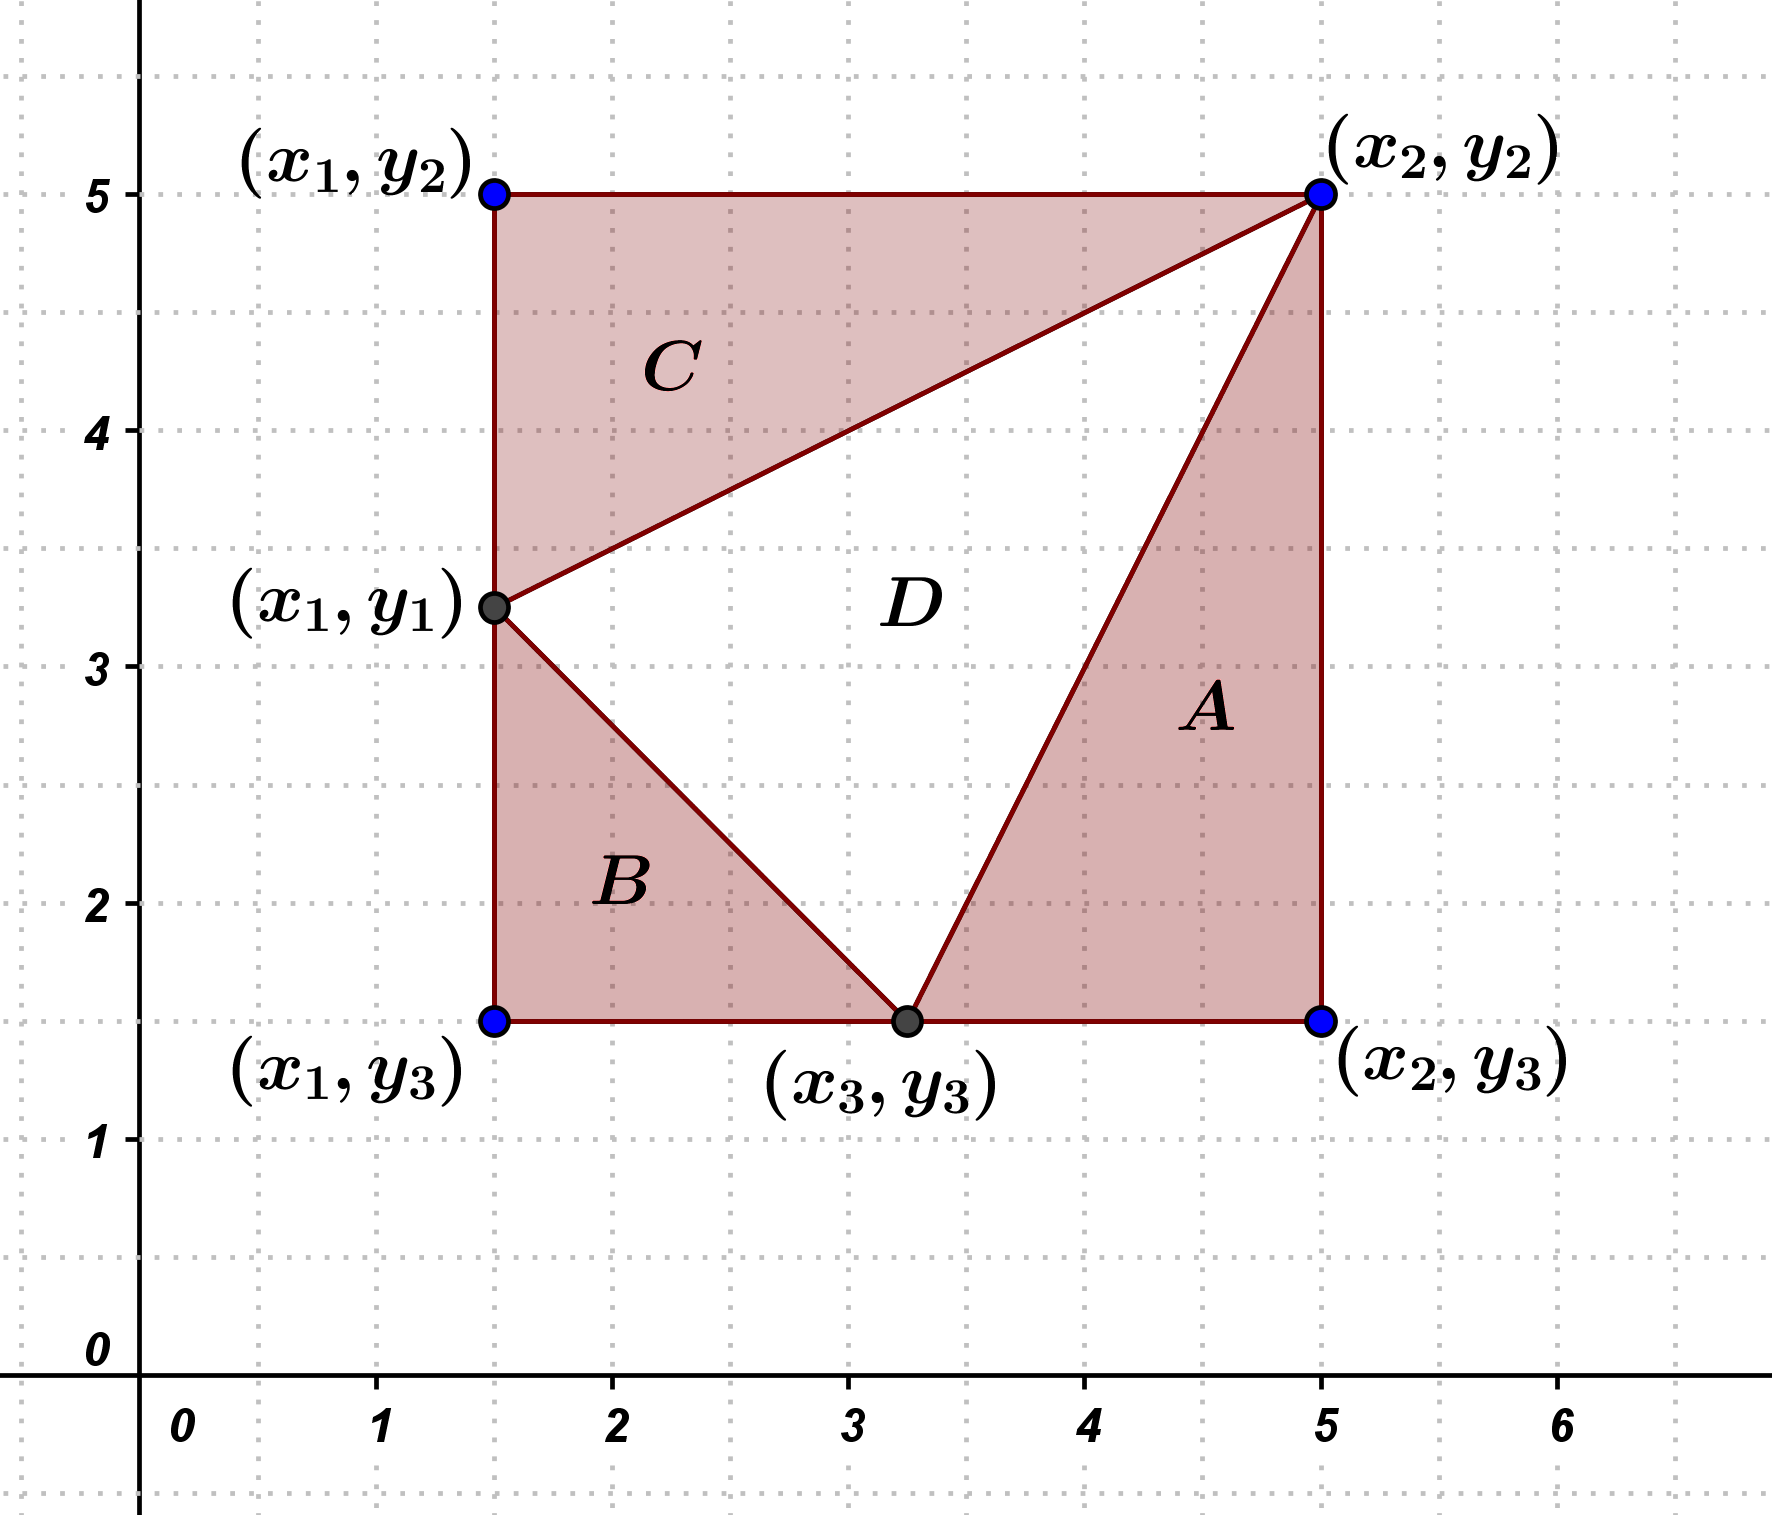
\includegraphics[width=.5\textwidth]{matarea.png}
\caption{A triangle on a cartesian coordinate}
\end{figure}

Our goal  is to find the area of $\triangle D(A_{\triangle D})$. But we can accomplish this just by subtracting the area of $\triangle A+\triangle B+\triangle C$ from the area of the $\square$.\\
Now, the area of $\square$ is
\begin{align*}
A_{\square}&=(x_2-x_1)(y_2-y_3)\\
           &=x_2y_2-x_2y_3-x_1y_2+x_1y_3
\end{align*}
The area of $\triangle A$ is given by
\begin{align*}
A_{\triangle A}&=\frac{1}{2}(x_2-x_3)(y_2-y_3)\\
                  &=\frac{1}{2}(x_2y_2-x_2y_3-x_3y_2+x_3y_3)
\end{align*}
And area of $\triangle B$ is given by
\begin{align*}
A_{\triangle B}&=\frac{1}{2}(x_3-x_1)(y_1-y_3)\\
                  &=\frac{1}{2}(x_3y_1-x_3y_3-x_1y_1+x_1y_3)
\end{align*}
Finally, the area of $\triangle C$ is given by
\begin{align*}
A_{\triangle C}&=\frac{1}{2}(x_2-x_1)(y_2-y_1)\\
                  &=\frac{1}{2}(x_2y_2-x_2y_1-x_1y_2+x_1y_1)
\end{align*}
Now,
\begin{align*}
A_{\triangle A}+A_{\triangle B}+A_{\triangle C}&=
\begin{cases}
\frac{1}{2}(x_2y_2-x_2y_3-x_3y_2+\hcancel[red]{x_3y_3})\\
+\frac{1}{2}(x_3y_1-\hcancel[red]{x_3y_3}-\hcancel[blue]{x_1y_1}+x_1y_3)\\
+\frac{1}{2}(x_2y_2-x_2y_1-x_1y_2+\hcancel[blue]{x_1y_1})
\end{cases}\\
&=x_2y_2+\frac{1}{2}(-x_2y_3-x_3y_2+ x_3y_1+x_1y_3-x_2y_1-x_1y_2)
\end{align*}
But we know that
\[A_{\triangle D} =A_{\square}-(A_{\triangle A}+A_{\triangle B}+A_{\triangle C})\]
Thus
\begin{align*}
A_{\triangle D} &= (\hcancel[red]{x_2y_2}-x_2y_3-x_1y_2+x_1y_3)-\bigl(\hcancel[red]{x_2y_2}+\frac{1}{2}(-x_2y_3-x_3y_2+ x_3y_1+x_1y_3-x_2y_1-x_1y_2)\bigl)\\
                &\ \ \vdots\tag{some algebraic simplification}\\
                &=\frac{1}{2}\bigl((x_3 y_2-x_2y_3)-(x_3y_1-x_1y_3)+(x_2y_1-x_1y_2)\bigl)\\
                &=\frac{1}{2}\left|
    \begin{matrix}
      x_1 & y_1 & 1\\
      x_2 & y_2 & 1\\
      x_3 & y_3 & 1
    \end{matrix}
    \right|
\end{align*}
\end{proof}
\begin{cor}
  If $\left|\begin{matrix}
      x_1 & y_1 & 1\\
      x_2 & y_2 & 1\\
      x_3 & y_3 & 1
    \end{matrix}
    \right|=0$, then the points $(x_1,y_1),( x_2,y_2)$ and $(x_3,y_3)$ lies on the same line that means they are collinear.
\end{cor}

\end{document}
